\documentclass{sig-alternate}
\usepackage{amsmath}
\usepackage[T1]{fontenc}
\usepackage{ae, aecompl}
\usepackage{color}
\usepackage{booktabs}
\usepackage{paralist}
\usepackage{graphicx}
\usepackage{amsfonts}
\usepackage{times}

\usepackage{float}
%\DeclareCaptionType{copyrightbox}
\usepackage[hyphens]{url}
\usepackage{enumerate}
\usepackage{algorithmicx}
\usepackage{algpseudocode}
\usepackage{algorithm}

\usepackage{subcaption}

\newcommand{\nn}{\nonumber}
\newcommand{\set}[1]{\mathcal{#1}}        			% Set
\newcommand{\rv}[1]{\boldsymbol{#1}}    			% Random variable
\renewcommand{\vec}[1]{\boldsymbol{\mathrm{#1}}} 	% Vector or Matrix
\newcommand{\event}[1]{\langle #1 \rangle}      	% Event
\newcommand{\arthur}[1]{\textcolor{blue}{Arthur: #1}}
\newcommand{\fixit}[1]{\textcolor{red}{#1}}
\newcommand{\etal}{\emph{et~al.}}


\renewcommand{\itemize}{\compactitem}
 \renewcommand{\enumerate}{\compactenum}

\newenvironment{mymathbox}
{\par\smallskip\centering\begin{lrbox}{0}%
\begin{minipage}[c]{0.8\textwidth}}
{\end{minipage}\end{lrbox}%
\framebox[0.9\textwidth]{\usebox{0}}%
\par\medskip
\ignorespacesafterend}
\begin{document}

%\title{Bitcoin Fraud with Targeted Blockchain Forks}
\title{Quantifying Web Adblocker Privacy}
%\title{Bitcoin Block and Transaction Withholding}
%\title{On Withholding Blocks and Transactions in Bitcoin}
%\title{Consequences of Withholding Blocks and Transactions in Bitcoin}
%\title{Consequences of Data Delivery Delay in Bitcoin}
%\title{Data Delivery Delay in Bitcoin}
%\numberofauthors{1}
\author{}
%\numberofauthors{1}
%\author{Arthur Gervais$^\dag$, Hubert Ritzdorf$^\dag$, Ghassan O. Karame$^\dag$, Srdjan Capkun$^\dag$\\ \medskip \affaddr{$^\dag$ETH Zurich, Switzerland} \\ \email{$^\dag$firstname.lastname@inf.ethz.ch} }

\numberofauthors{1}
%\author{$^\dag$, $^\dag$, $^\ddag$ and $^\dag$\\ \medskip \affaddr{$^\dag$ETH Zurich, Switzerland \\ \email{$^\dag$firstname.lastname@inf.ethz.ch }

\maketitle

\begin{abstract}
\end{abstract}

\section{Introduction} \label{sec:introduction}

 Our contributions in this paper can be summarized as follows:
 \begin{itemize}
 \item We examine the temporal evolution of the tracking behavior for a fixed set of websites over a period of 3 months.
 \item We investigate how much exposed a device with Mobile User Agent is compared to a Desktop device.
 \item We enhance the metrics used for the assessment by augmenting them with WHOIS-entity information.
 \item Additionally to the existing metrics, we examine the worst-case scenarios in terms of privacy compromise.
 \item We perform our evaluation taking into consideration not only the top 500 most-visited domains, but also 500 additional and uniformly-selected ones.
 \end{itemize}

\section{Background} \label{sec:background}
The literature employed the number of blacklisted domains as a privacy indication~\cite{XX}, but we argue that this is not a sufficient indicator for the offered privacy enhancements. Instead of only capturing the reduction in percentage of accessed third parties, we argue that the graph of third parties should be analyzed in its entirety. Certain third parties are furthermore clearly collaborating, since they belong to the same logical entity. We therefore define the following privacy metrics in order to objectively compare different adblocker.

{\color{red}Please elaborate on the background. }

\section{Privacy metrics} \label{sec:privacy_metrics}
In this Section we introduce the privacy metrics used in order to quantify the privacy provisions of adblocker.

%{\color{blue}We model the tracking of a user $U$ through third parties as undirected graph $G=(E,V)$, where $E$ are edges, and $V$ vertices. A vertice can represent either a first party \emph{fp} (i.e. the URL the user visits) or a third party \emph{tp} (i.e. the URL of a resource that a first party fetches). An edge is built between a \emph{fp} that fetches a \emph{tp}. By visiting a series of websites $S_U = \{w_1, w_2, .. , w_n\}$, the complete tracking graph $G$ becomes apparent.}

\subsection{Request graph} \label{sec:graph_definition}
We model the tracking of a user $U$ through third parties as undirected graph $G=(E,V)$, where $E$ are edges, and $V$ vertices. A vertex $V_S$ represents a domain and is connected to another vertex $V_T$ through an edge $E$, if and only if at least one request has been sent from $V_S$ to $V_T$. In that case, $V_S$ is the \textit{source} of the request and $V_T$ the \textit{target} of the request.

In the following, we use the term \textit{third-party request} (TPR) to denote the requests that are sent to a target domain $T$ that differs from the source domain $S$ and corresponds to a graph edge $E$ between the nodes $V_S$ and $V_T$. On the contrary, the requests whose source and target coincide are designated as \textit{first-party requests} (FPR) and are not taken into consideration for the construction of $G$.

The source and the target domain are referred to as \textit{first-party domain} (FPD) and \textit{third-party domain} (TPD) and correspond to FPD and TPD graph nodes, $V_S$ and $V_T$, respectively.

We augment \emph{G} by incorporating the logical relationship between third party domains. Two \emph{tp}, belonging to the same logical entity are thus combined into one vertice, resulting in a hierarchical graph. Figure~\ref{fig:graph} visualizes the different components of the build graph. Given \emph{G}, we evaluate the respective privacy provisions based on the following metrics.

\begin{figure}[htb!]
  \centering
  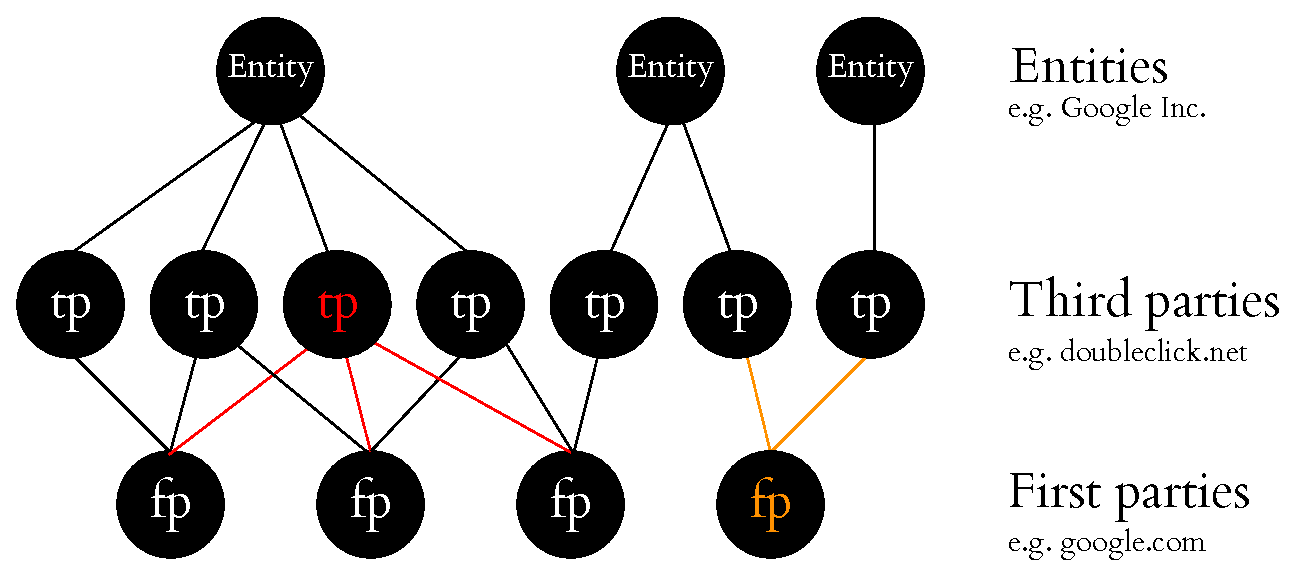
\includegraphics[width=0.45\textwidth]{figures/graph.eps}
  \caption{Graph built based on the regular crawling of the respective first parties. The colored third party has a node degree of 3, the colored first party has a node degree of 2.}\label{fig:graph}
\end{figure}

\subsection{Metrics}
\paragraph{Degree of first party}
The degree of a FPD node of graph $G$ refers to the number of TPDs that it has sent at least one third-party request to. That is, the more edges a FPD node has --or, equivalently, the more third parties loaded by a first-party-- the more exposed to tracking the user is while visiting this website. Henceforth, the comparison of the FPD-node degrees provides a metric to evaluate directly the impact on the privacy that an adblocker has.

\paragraph{Degree of third party}
The degree of a TPD node can be directly translated to the number of first-party websites that this third party exchanges information with and it thence potentially tracks. The frequency with which a third party is requested by the websites $S_U$ that a user $U$ visits, determines the tracking power of this particular third party, as well as the ensuing privacy concerns for $U$.
Clearly, the more often a third party is accessed over the user's series of websites $S_U$, the less privacy the user experiences from this particular third party. To exemplify this statement, let's assume that a third party is requested by only one of the first-party websites $S_U$ visited by $U$. This third party will in this case learn that the user has accessed the respective first party, but has a limited view of their browsing behavior. If the third party, however, is requested by over 80\% of the user's visited websites, $S_U$, the third party will likely be able to recover 80\% of the web behavior of $U$.

We capture this privacy notion by assessing the degree of the TPD nodes in the graph $G$ so as to evaluate the improvement that the ad-blocking software can achieve.

\paragraph{Graph density}
In addition to the outlined privacy metrics, we consider the graph density of $G$. Since an edge on the graph $G$ represents a tracking relationship between a third and a first party, we expect that the denser the graph $G$, the more information (can be retrieved by third parties/can leak to third parties) with respect to the browsing behavior of the user. We observer that the more dense $G$ is, the more third parties are likely to be able to track the user $U$. The graph density therefore allows to reason about the possible privacy improvements by the respective ad-blocking software. For undirected graphs, the graph density is commonly defined as:
\begin{equation}
D = \frac{2 |E|}{|V|(|V|-1)}
\end{equation}

Note that we cannot achieve the maximum density of 1, because the first parties in $G$ are not directly connected, because according to our definition in Section \ref{sec:graph_definition}, the FPD nodes cannot be directly connected.

\paragraph{Blacklist latency}
The formerly presented metrics only allow us to reason about the privacy provisions of the advertisement blocking software at a given time $t$. The advertisement industry, however, operates dynamically by using e.g., new advertisement techniques and new third party URLs. In order to capture the temporal privacy provisions of the adblocker, we evaluate the the aforementioned privacy metrics over a timespan of several months. This allows us to reason quantitatively about how fast an adblocker adapts to a changing advertisement environment.

\subsection{Beyond URLs}
The metrics examined so far capture the tracking behavior by raw third party domains. Since the URL information, however, does not encapsulate many aspects of the respective web infrastructure and resulting privacy risks, we augment the graph $G$, by incorporating, logical entities, cookies, and whether a third party contains active or passive content.

\paragraph{Logical entity}
\label{sec:logical_entity}
Instead of focusing on the URL of a third party, we link the third parties based on their respective owner information. Third parties such as \url{doubleclick.net} and \url{google.com} for example are both owned by the same entity Google Inc. Their collusion therefore seems more likely, and affects the privacy of a web user $U$ more significantly, than if both were belonging to two different logical entities. By incorporating the logical relation among third party domains, we therefore capture a more realistic privacy leakage through user web surf activity.

\paragraph{DNT influence}
Does DNT change something (has been studied before).

\section{Evaluation}
In this section, we explain in detail our experimental setup, discuss the extracted results and followingly examine the impact of the parameters from a privacy viewpoint.

\subsection{Experimental setup}
\subsubsection{Lightbeam first-partyness heuristics}
The distinction between FPRs and TPRs is crucial in our attempt to precisely quantify the ad-blocking efficiency for each user profile $U$, since they define the exact topology of the derived graph $G$.

Although Lightbeam already implements an algorithm to decide over the ``first-partyness'' of a request, so as to create this graph, it does not have the exact knowledge of the actual website visited. To compensate for this lack of information, Lightbeam applies some heuristics in order to estimate which source domain initiated the request, compares it to the already-known target domain of the request and followingly classifies it as a FPR or TPR.

Nonetheless, this classification is not always in accordance with our definitions of FPR and TPR, as introduced in Section \ref{sec:privacy_metrics}. By examining the request logs after a complete crawl cycle and comparing the estimated source to the actual crawled domain, two types of false-positive cases (Table \ref{table:false_positive_examples}) arise:

\begin{itemize}
\item \textbf{Unrecognized TPRs:} The request is mistakenly considered to be a FPR according to the Lightbeam heuristics, this way ``hiding'' a TPR edge from the graph.
\item \textbf{Misclassified TPRs:} The request is correctly found to be a TPR, but not for the correct FPD node, i.e. the one corresponding to the actually crawled domain. The inaccuracy introduced to the graph results from the potential introduction of a bogus FPD node, as well as the false number of TPR edges starting from the correct and the bogus FPD nodes.
\end{itemize}

As results from the experimental evaluation on the data of one full crawl cycle (1000 visited first parties) and 12 different user profiles, the misclassified and unrecognized TPRs make up for 2.0\%-12.0\% and 4.0\%-11.0\% of the total requests, accordingly. The percentages differ for the various user profiles examined.

\begin{table}
\centering
\small
\begin{tabular}{|c|c c c|}
\hline
& Visited Domain & Estimated Source & Target \\
\hline
Recognized & wp.pl & wp.pl & facebook.com \\
Misclassified & wp.pl & facebook.com & fbcdn.net \\
Unrecognized & wp.pl & facebook.com & facebook.com \\
\hline
\end{tabular}
\caption{Examples of misclassified and unrecognized TPRs}
\label{table:false_positive_examples}
\end{table}

\subsubsection{Methodology}
In this subsection, we outline the experimental setup and the corresponding results.

\paragraph{User profiles}
\label{sec:user_profiles}
In order to compare the efficacy of different adblockers, as well as the influence of different browser settings on their adblocking efficiency, we create 12 user profiles, $U$, each of which is defined as a combination of the following parameters (Table \ref{table:user_profiles}):

\begin{itemize}
 \item Ad-blocker installed
 \item Block policy: The blacklists applied or the list of blocked trackers is set to its default state or set so as to provide a maximal protection
 \item Mobile or Desktop User Agent
 \item Do Not Track (DNT) header enabled
\end{itemize}


\paragraph{Crawled URLs}
\label{sec:crawled_urls}
An appropriate criterion for the evaluation of an adblocker is its performance in the most frequent case. Consequently, it would be plausible to test its efficiency for the \textit{500 domains with the highest incoming web traffic}. Nonetheless, considering only the top-visited domains in our evaluation would imply the risk of favoring an adblocker optimized to perform better for a certain group of websites, eventually biasing our experimental results. An appropriate countermeasure would hence be to extend our URL sample set with another \textit{500 uniformly-selected domains} (randomly-chosen according to a uniform distribution) among the top 1 million most-visited domains. The sample set $S$ of 1000 URLs is extracted using the Alexa Traffic Rank as a reference point and is stored and kept unchanged throughout the whole evaluation period, so as to decorrelate any variations of the results between two different days from the selection of the sample set $S$.

Since nowadays most of the web applications are based on asynchronous calls to fetch data, when the DOM has finished rendering, only a part of the content has been downloaded in most of the cases, or equivalently, not all of the requests have been sent to any first or third parties to fully load the page content. Therefore, to collect the complete data and better simulate the common user browsing behavior, the crawler waits 20 seconds on each website of our sample set $S$ and record any requests sent, before closing it and proceeding to the next domain. Additionally, to achieve independency from any heuristics in our attempt to determine the source of a request, we augment the request data provided by \textit{Lightbeam} with the actual knowledge of the currently visited first-party.

Last but not least, in order to decouple the experiment conditions from the influence of any time- or location-related effects --i.e. variations of the served content, locale-based personalization-- all user profiles $U$ execute the same crawling routine simultaneously, whilst running on the same machine, thus behind the same IP address, Browser and Operating System. However, some of the instances are configured to send their requests with a User-Agent HTTP header that corresponds to a mobile device (iPhone with iOS 6), with the aim that we can extend our observations for the mobile users.

\subsection{Experimental Results}
In the present, we discuss the outcome of the experiments, i.e. the performance of the different user profiles and metrics, so as to lay the foundations for the ensuing conclusions regarding the influence of the individual parameters.

For a more effective overview of the experimental results for each user profile $U$, the following conventions are used in the Figure \ref{fig:metrics_without_entities}:
\begin{itemize}
 \item The \textit{color} denotes the adblocker installed.
 \item The \textit{line width} indicates the protection degree --i.e. default settings as opposed to the maximal protection achieved through the use of maximum block policy or the DNT header.
 \item Profiles with Mobile User Agent are plotted in \textit{dashed lines}.
\end{itemize}
The data collected for user profile $U$ on a specific date correspond to a different graph $G$. The plot legends corresponding to each user profile $U$ are listed in more detail in Table \ref{table:user_profiles}.

  % Defining dash lines
  \newcommand\solidthinrule[1][.5cm]{\rule[0.5ex]{#1}{.4pt}}
  \newcommand\solidthickrule[1][.5cm]{\rule[0.5ex]{#1}{1.5pt}}
  \newcommand\dashedthinrule{\mbox{%
    \solidthinrule[1mm]\hspace{1mm}\solidthinrule[1mm]\hspace{1mm}\solidthinrule[1mm]}}
  \newcommand\dashedthickrule{\mbox{%
    \solidthickrule[1mm]\hspace{1mm}\solidthickrule[1mm]\hspace{1mm}\solidthickrule[1mm]}}
  \definecolor{darkgreen}{rgb}{0, 0.8, 0}

  \begin{table*}
  \centering
  \begin{tabular}{|c|c c c c c|}
  \hline
  User Profile & Adblocker & Block Policy & DNT & User Agent & Legend \\
  \hline
  Ghostery\_Default & Ghostery & Default & No & Desktop  & {\color{red}\solidthinrule} \\
  Ghostery\_MaxProtection & Ghostery & Max & No & Desktop & {\color{red}\solidthickrule} \\
  Adblockplus\_Default & AdblockPlus & Default & No & Desktop & {\color{blue}\solidthinrule} \\
  Adblockplus\_MaxProtection & AdblockPlus & Max & No & Desktop & {\color{blue}\solidthickrule} \\
  NoAdblocker & None & - & No & Desktop & {\color{darkgreen}\solidthinrule} \\
  NoAdblocker\_DNT & None & - & Yes & Desktop & {\color{darkgreen}\solidthickrule} \\
  Ghostery\_Default\_MUA & Ghostery & Default & No & Mobile & {\color{red}\dashedthinrule} \\
  Ghostery\_MaxProtection\_MUA & Ghostery & Max & No & Mobile & {\color{red}\dashedthickrule} \\
  Adblockplus\_Default\_MUA & AdblockPlus & Default & No & Mobile & {\color{blue}\dashedthinrule} \\
  Adblockplus\_MaxProtection\_MUA & AdblockPlus & Max & No & Mobile & {\color{blue}\dashedthickrule} \\
  NoAdblocker\_MUA & None & - & No & Mobile & {\color{darkgreen}\dashedthinrule} \\
  NoAdblocker\_DNT\_MUA & None & - & Yes & Mobile & {\color{darkgreen}\dashedthickrule} \\
  \hline
  \end{tabular}
  \caption{Overview of user profiles examined}
  \label{table:user_profiles}
  \end{table*}

  \begin{figure}
   \centering

   \begin{subfigure}{.45\textwidth}
    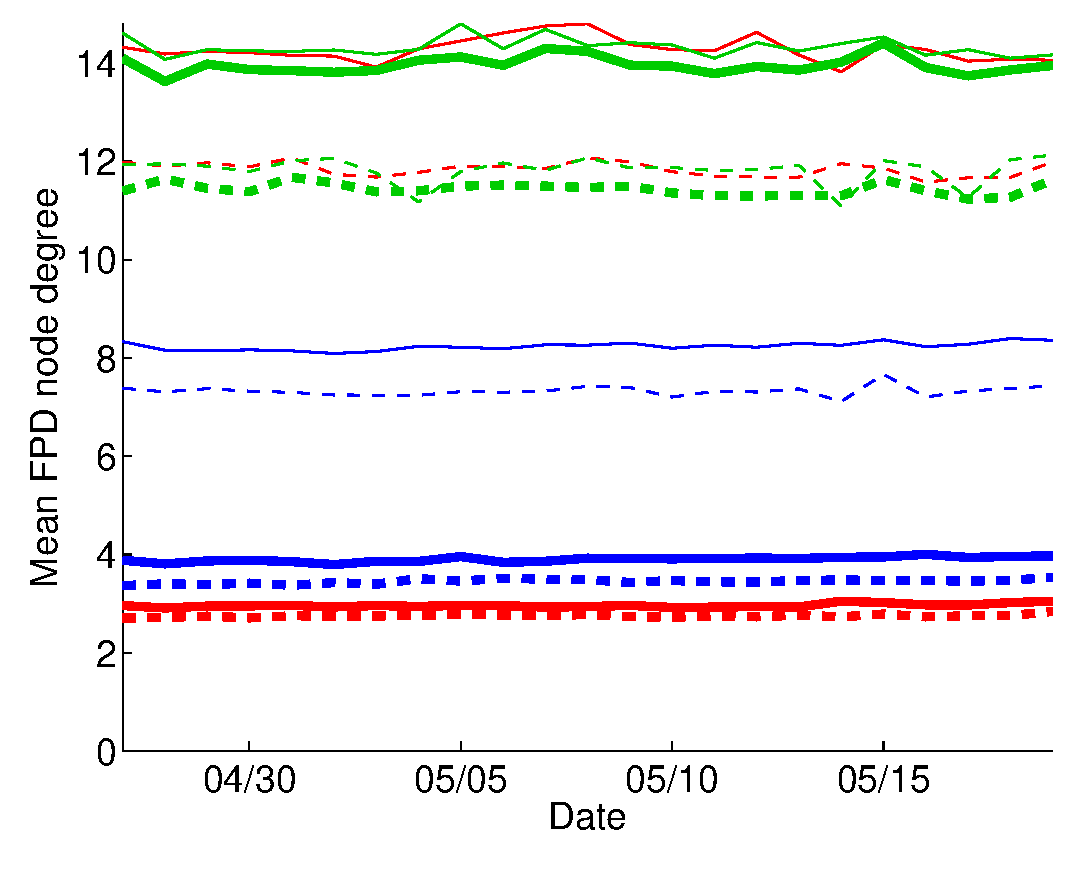
\includegraphics[width=\textwidth]{figures/plots/first-means.eps}
    \caption{Mean value of the degree of the FPD nodes, $V_S$ over time for each user profile $U$}
    \label{fig:first_means}
  \end{subfigure}

  \begin{subfigure}{.45\textwidth}
    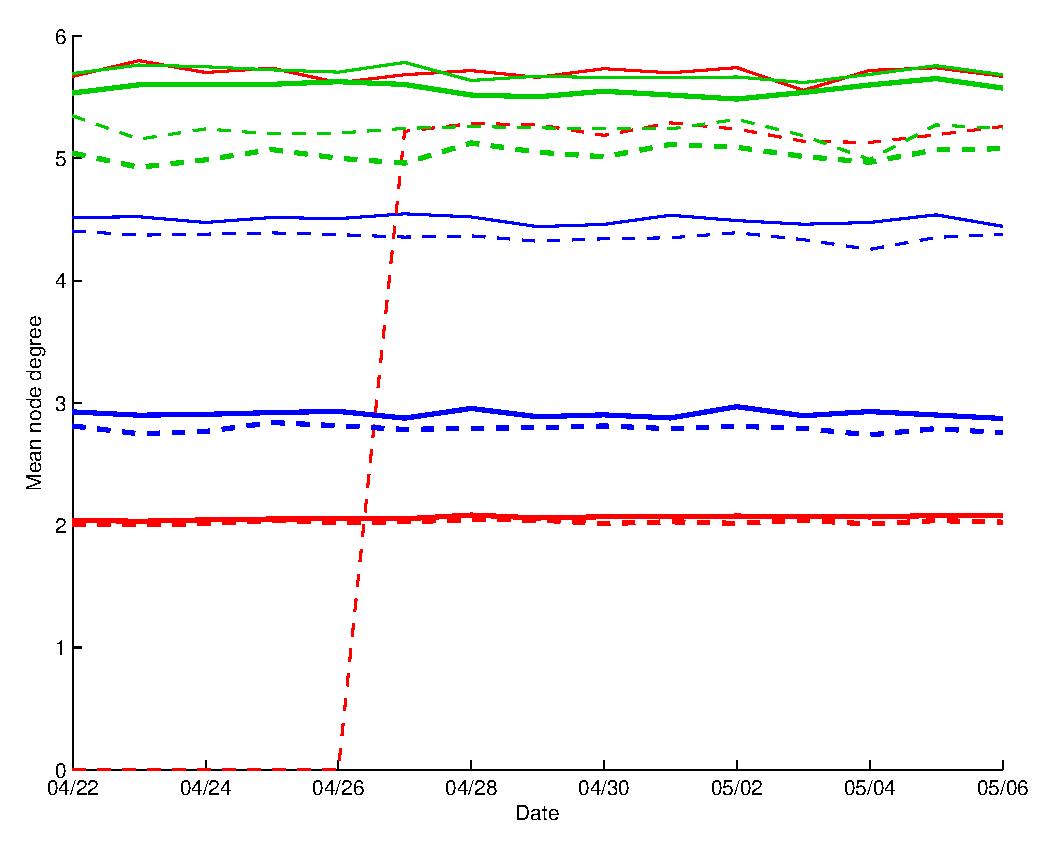
\includegraphics[width=\textwidth]{figures/plots/third-means.eps}
    \caption{Mean value of the degree of the TPD nodes, $V_T$ over time for each user profile $U$}
    \label{fig:third_means}
  \end{subfigure}

  \begin{subfigure}{.45\textwidth}
    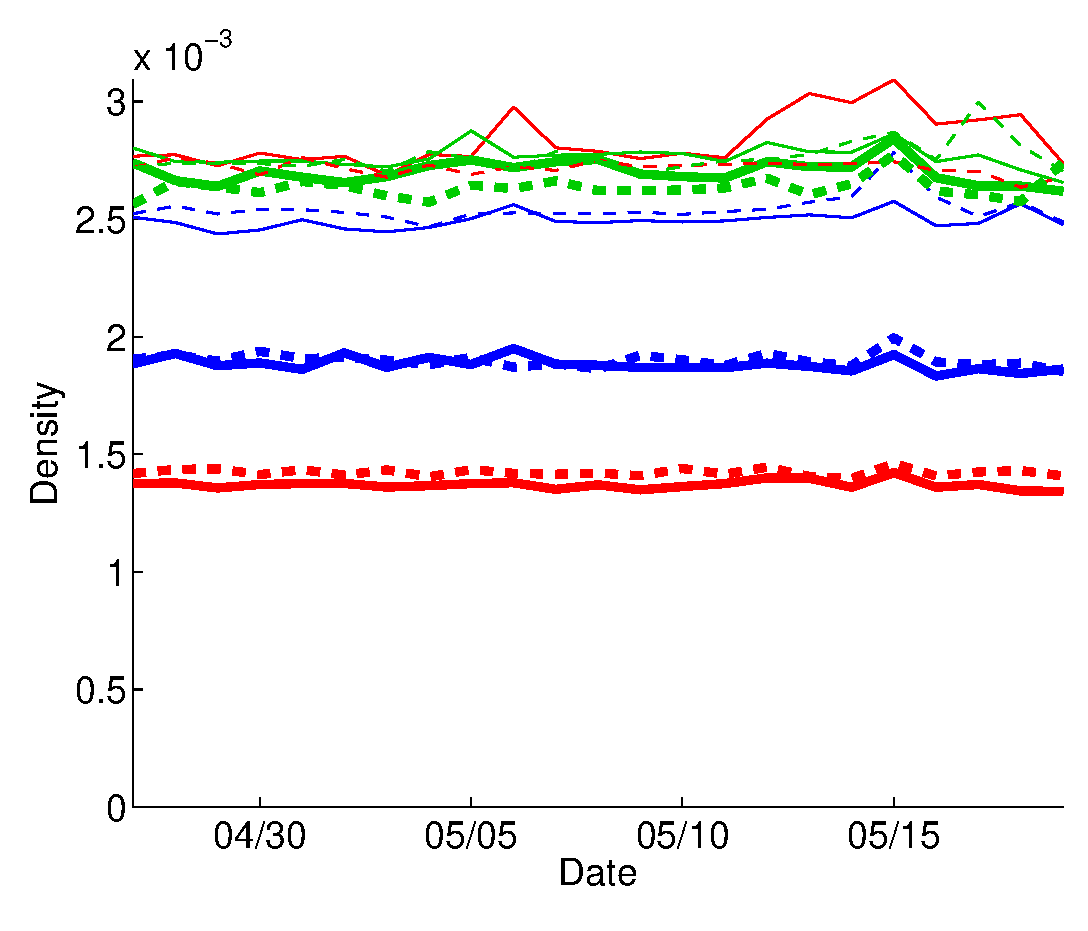
\includegraphics[width=\textwidth]{figures/plots/density.eps}
    \caption{Density of graph $G$ over time for each user profile $U$}
    \label{fig:density}
  \end{subfigure}

  \caption{Time evolution of the metrics \textbf{\textit{without}} domain grouping according to entities.}
  \label{fig:metrics_without_entities}
  \end{figure}

\begin{figure}
   \begin{subfigure}{.45\textwidth}
    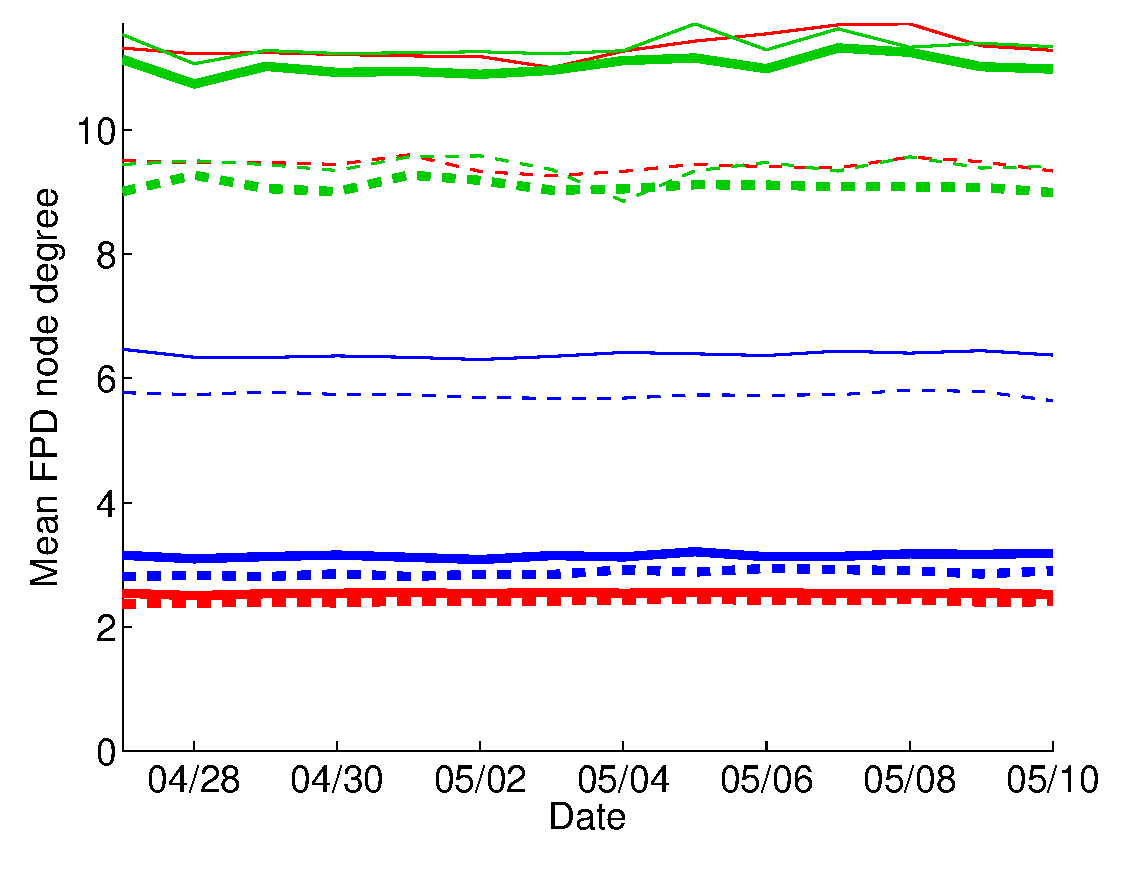
\includegraphics[width=\textwidth]{figures/plots/first-means-entities.eps}
    \caption{Mean value of the degree of the FPD nodes, $V_S$ over time for each user profile $U$}
    \label{fig:first_means_entities}
  \end{subfigure}

  \begin{subfigure}{.45\textwidth}
    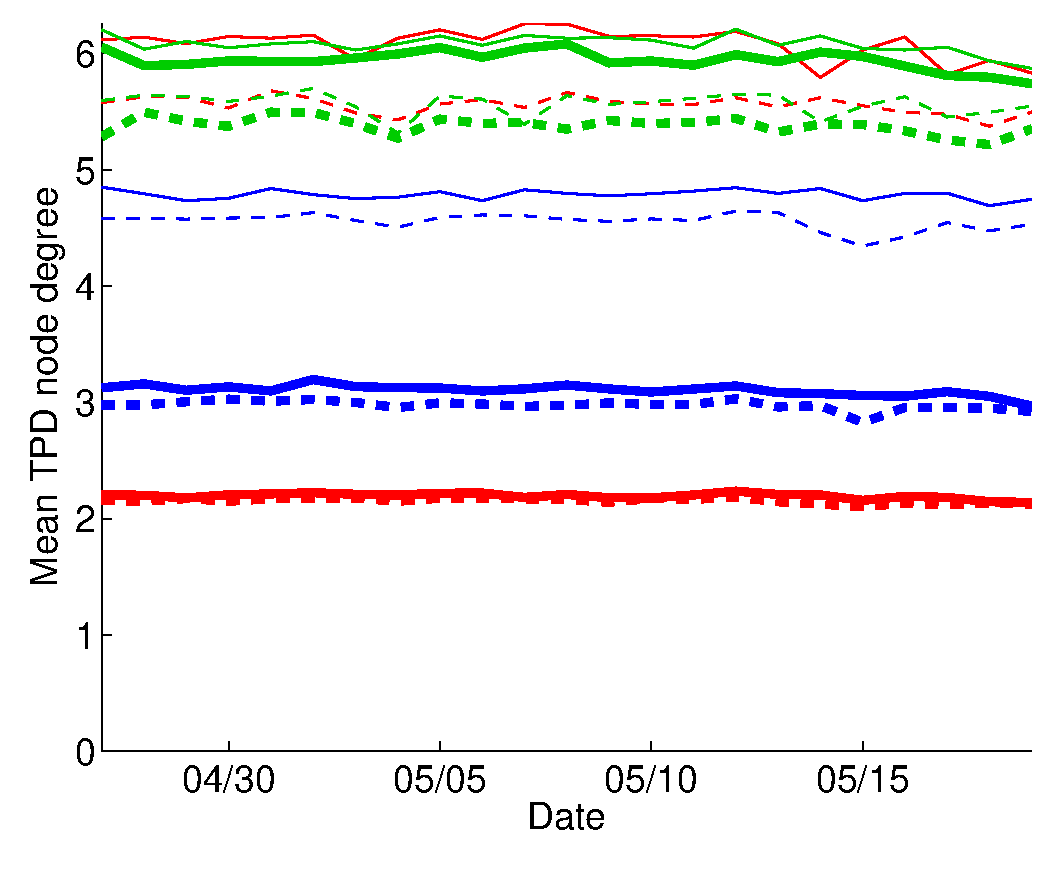
\includegraphics[width=\textwidth]{figures/plots/third-means-entities.eps}
    \caption{Mean value of the degree of the TPD nodes, $V_T$ over time for each user profile $U$}
    \label{fig:third_means_entities}
  \end{subfigure}

  \begin{subfigure}{.45\textwidth}
    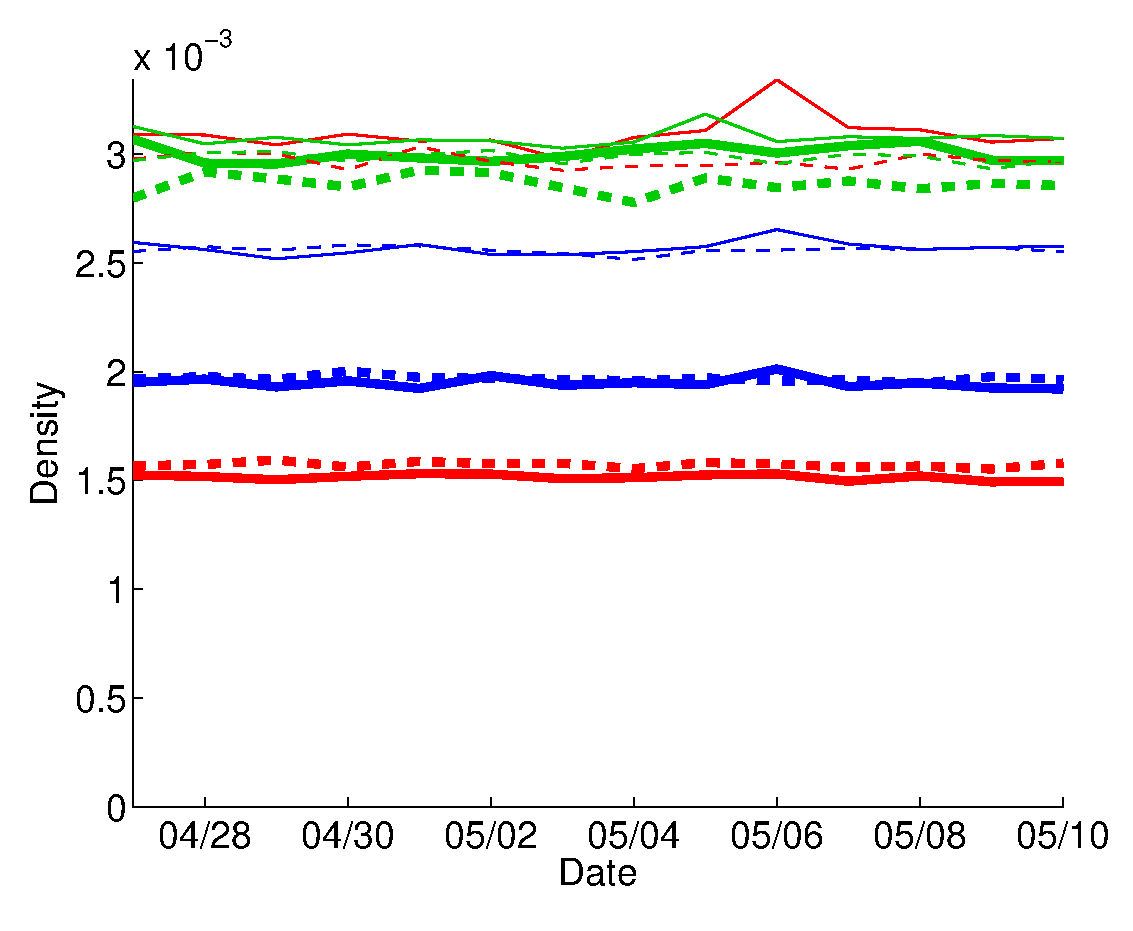
\includegraphics[width=\textwidth]{figures/plots/density-entities.eps}
    \caption{Density of graph $G$ over time for each user profile $U$}
    \label{fig:density_entities}
  \end{subfigure}
  \caption{Time evolution of the metrics \textbf{\textit{with}} domain grouping according to entities.}
  \label{fig:metrics_with_entities}
  \end{figure}

    \begin{figure*}
   \centering
   \begin{subfigure}{.38\textwidth}
    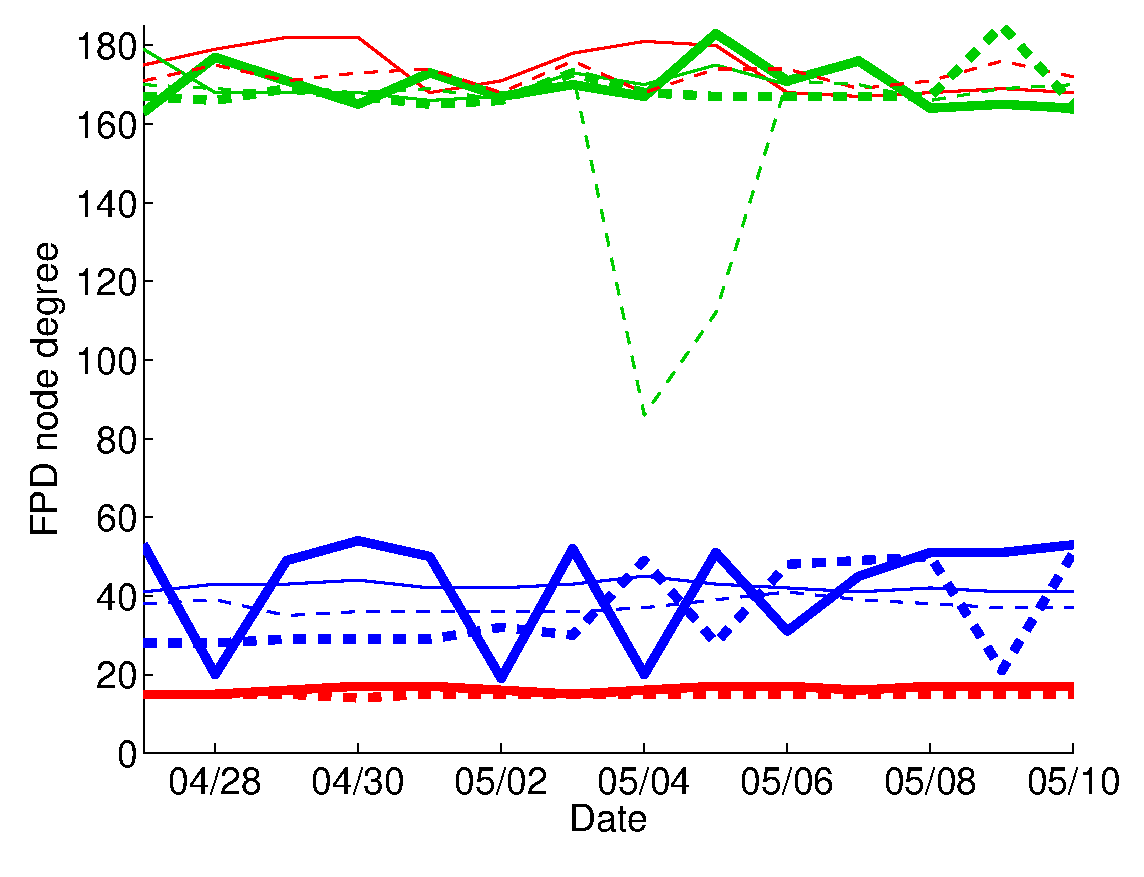
\includegraphics[width=\textwidth]{figures/plots/first-mean-top1.eps}
    \caption{Highest degree of FPD nodes, $V_S$ over time for each user profile $U$}
    \label{fig:first_mean_top1_without_entities}
  \end{subfigure}
  \begin{subfigure}{.38\textwidth}
    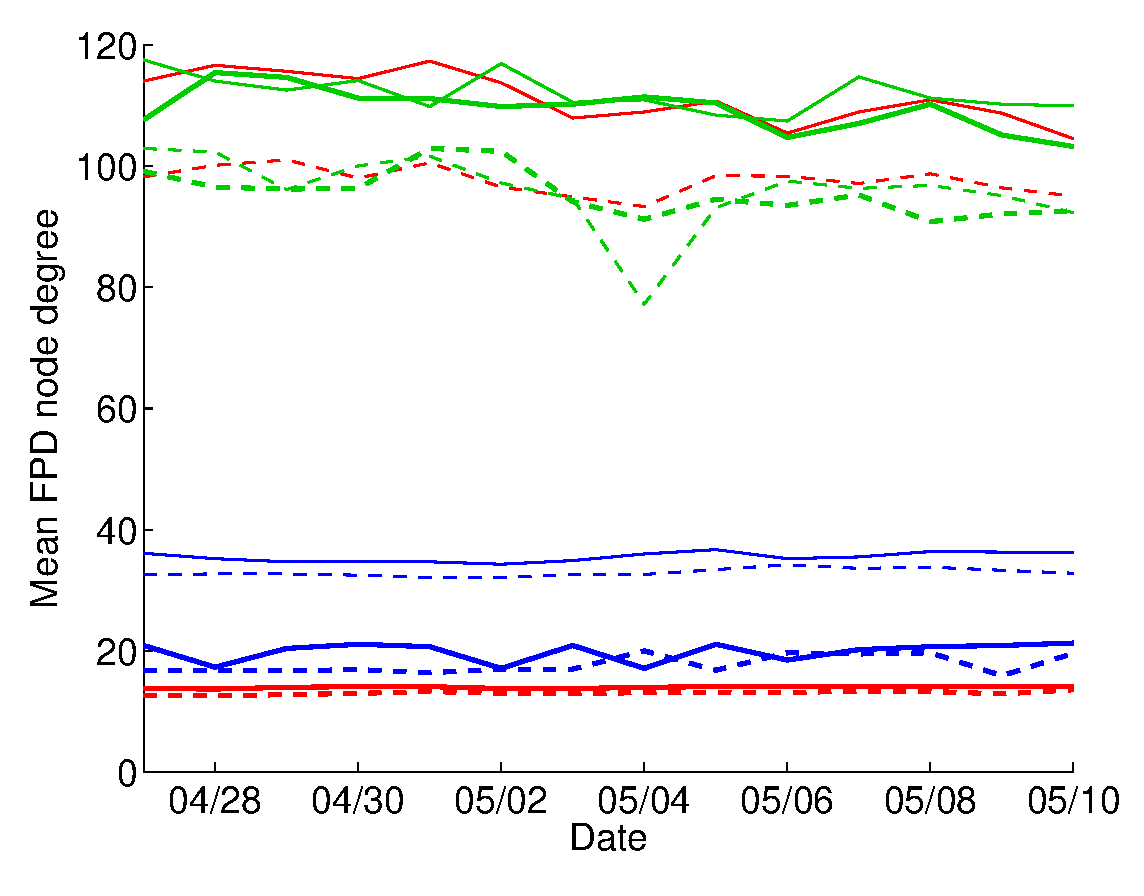
\includegraphics[width=\textwidth]{figures/plots/first-mean-top10.eps}
    \caption{Mean value of the degree of the 10 most-connected FPD nodes, $V_T$ over time for each user profile $U$}
    \label{fig:first_mean_top10_without_entities}
  \end{subfigure}
  \begin{subfigure}{.38\textwidth}
    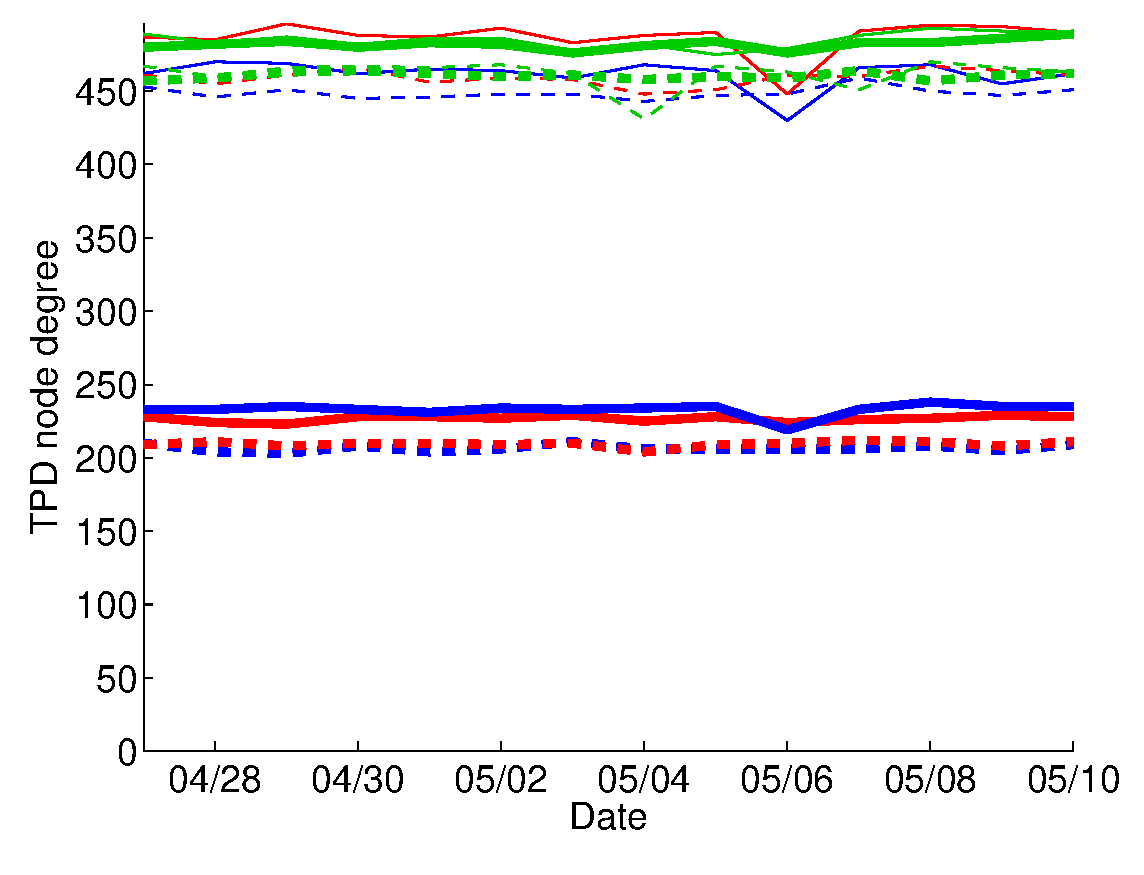
\includegraphics[width=\textwidth]{figures/plots/third-mean-top1.eps}
    \caption{Highest degree of TPD nodes, $V_T$ over time for each user profile $U$}
    \label{fig:third_mean_top1_without_entities}
  \end{subfigure}
  \begin{subfigure}{.38\textwidth}
    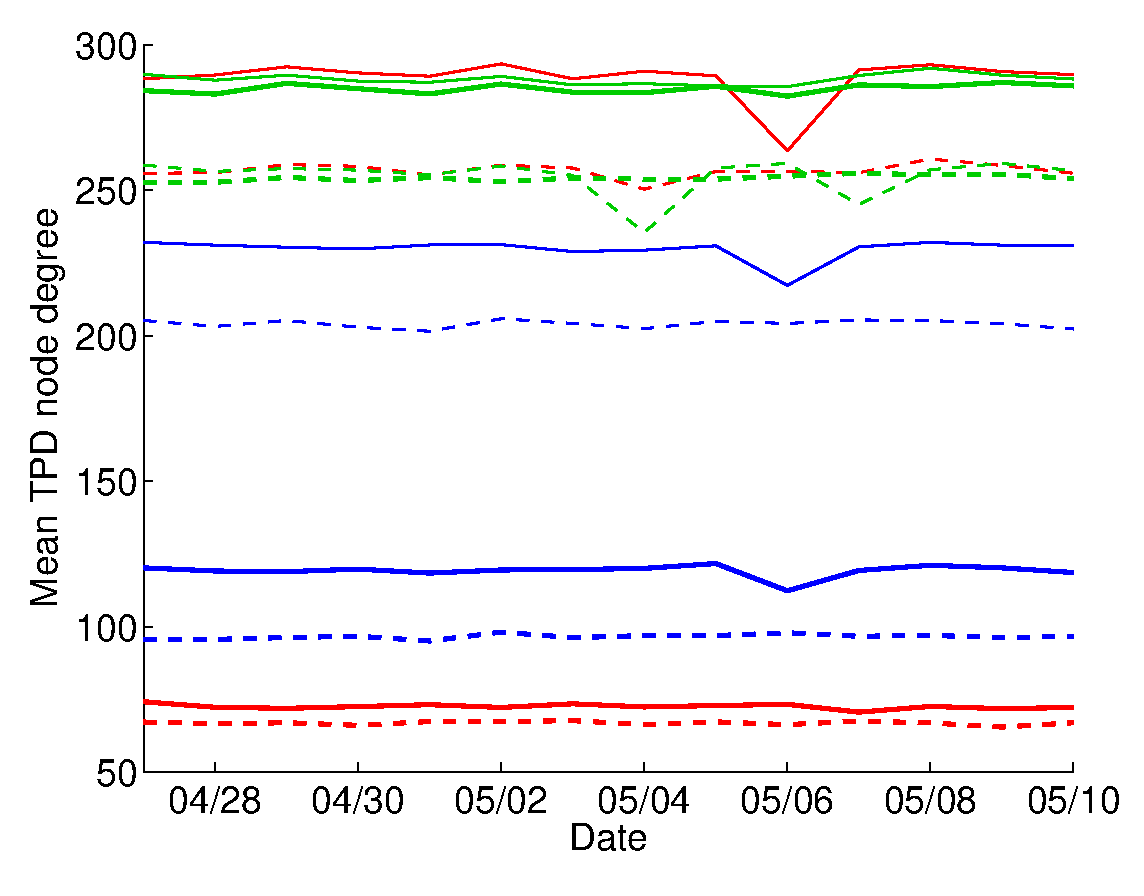
\includegraphics[width=\textwidth]{figures/plots/third-mean-top10.eps}
    \caption{Mean value of the degree of the 10 most-connected TPD nodes, $V_T$ over time for each user profile $U$}
    \label{fig:third_mean_top10_without_entities}
  \end{subfigure}

%  \caption{Time evolution of the first and third-party degree metrics for the most-connected FPD and TPD nodes, accordingly \textbf{\textit{without}} domain grouping according to entities.}
%  \label{fig:highest_degree_nodes_without_entities}
%  \end{figure}

%  \begin{figure}
%   \centering
   \begin{subfigure}{.38\textwidth}
    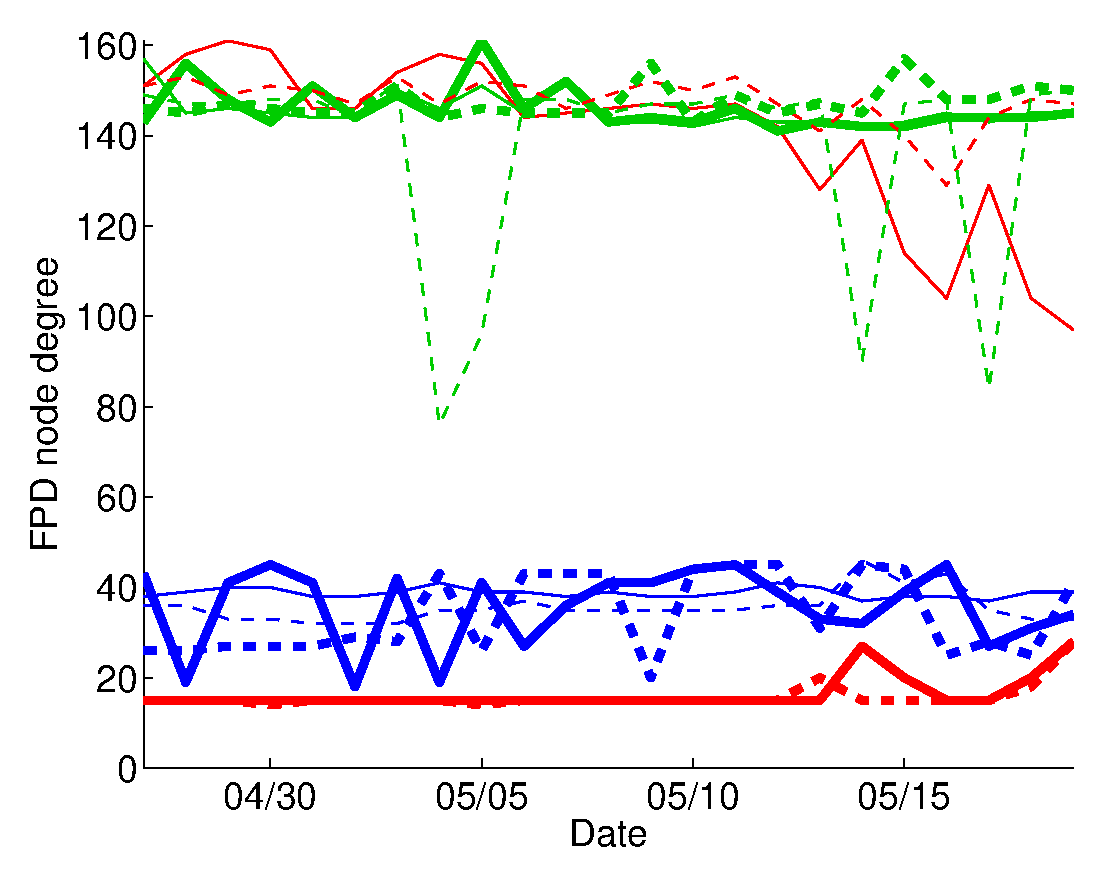
\includegraphics[width=\textwidth]{figures/plots/first-mean-top1-entities.eps}
    \caption{Highest degree of FPD nodes, $V_S$ over time for each user profile $U$}
    \label{fig:first_mean_top1_with_entities}
  \end{subfigure}
  \begin{subfigure}{.38\textwidth}
    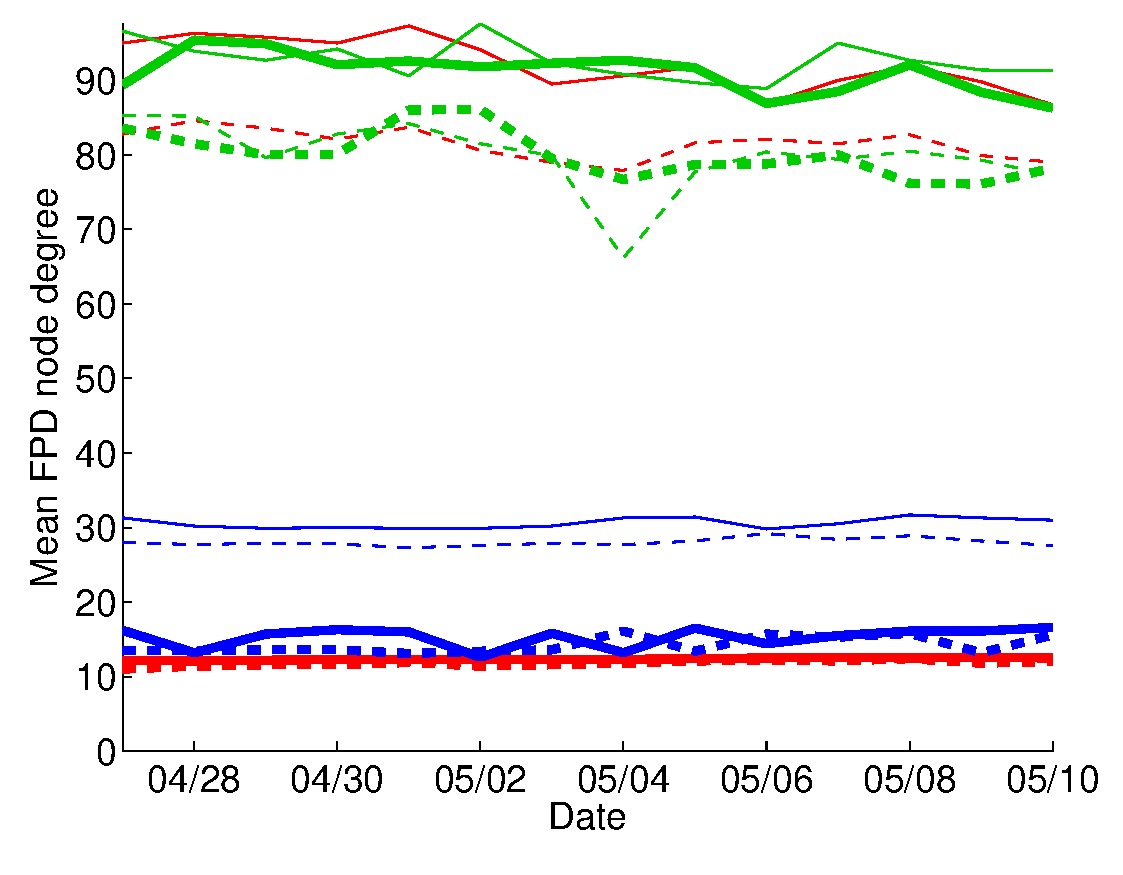
\includegraphics[width=\textwidth]{figures/plots/first-mean-top10-entities.eps}
    \caption{Mean value of the degree of the 10 most-connected FPD nodes, $V_T$ over time for each user profile $U$}
    \label{fig:first_mean_top10_with_entities}
  \end{subfigure}
  \begin{subfigure}{.38\textwidth}
    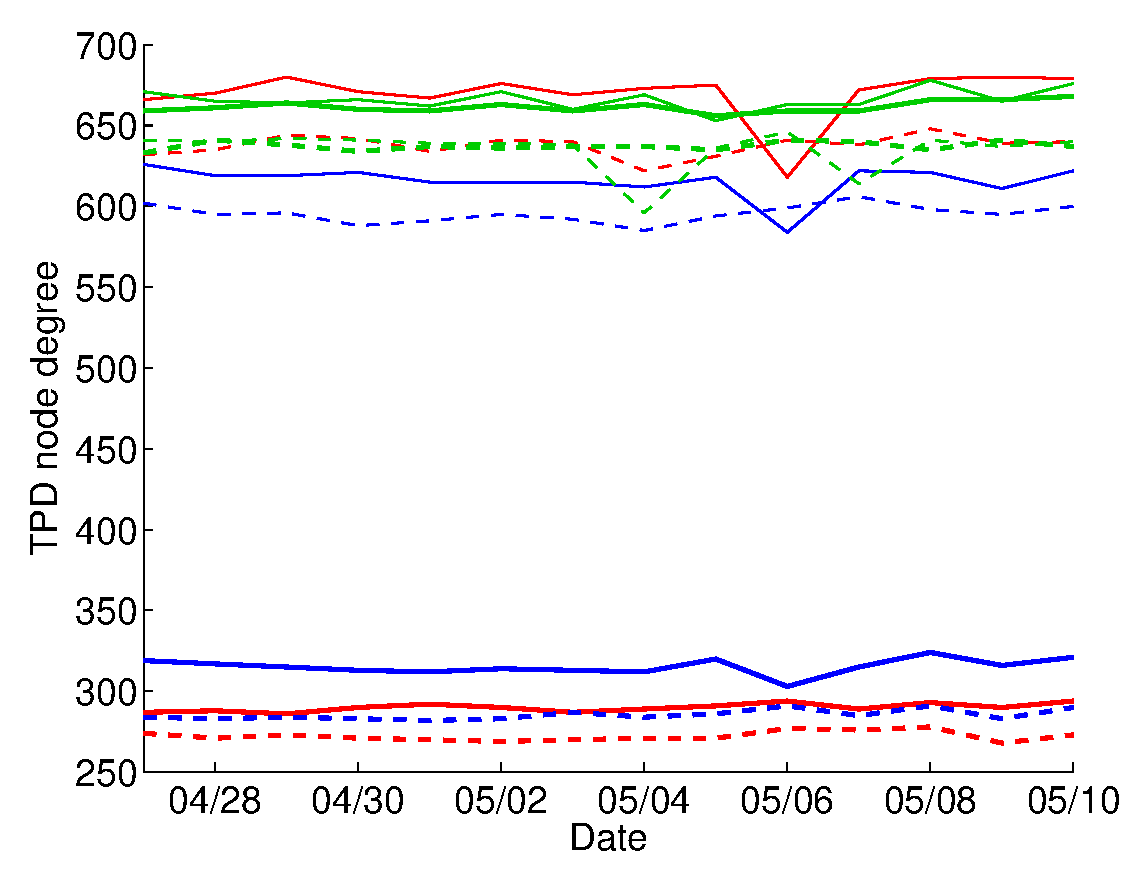
\includegraphics[width=\textwidth]{figures/plots/third-mean-top1-entities.eps}
    \caption{Highest degree of TPD nodes, $V_T$ over time for each user profile $U$}
    \label{fig:third_mean_top1_with_entities}
  \end{subfigure}
  \begin{subfigure}{.38\textwidth}
    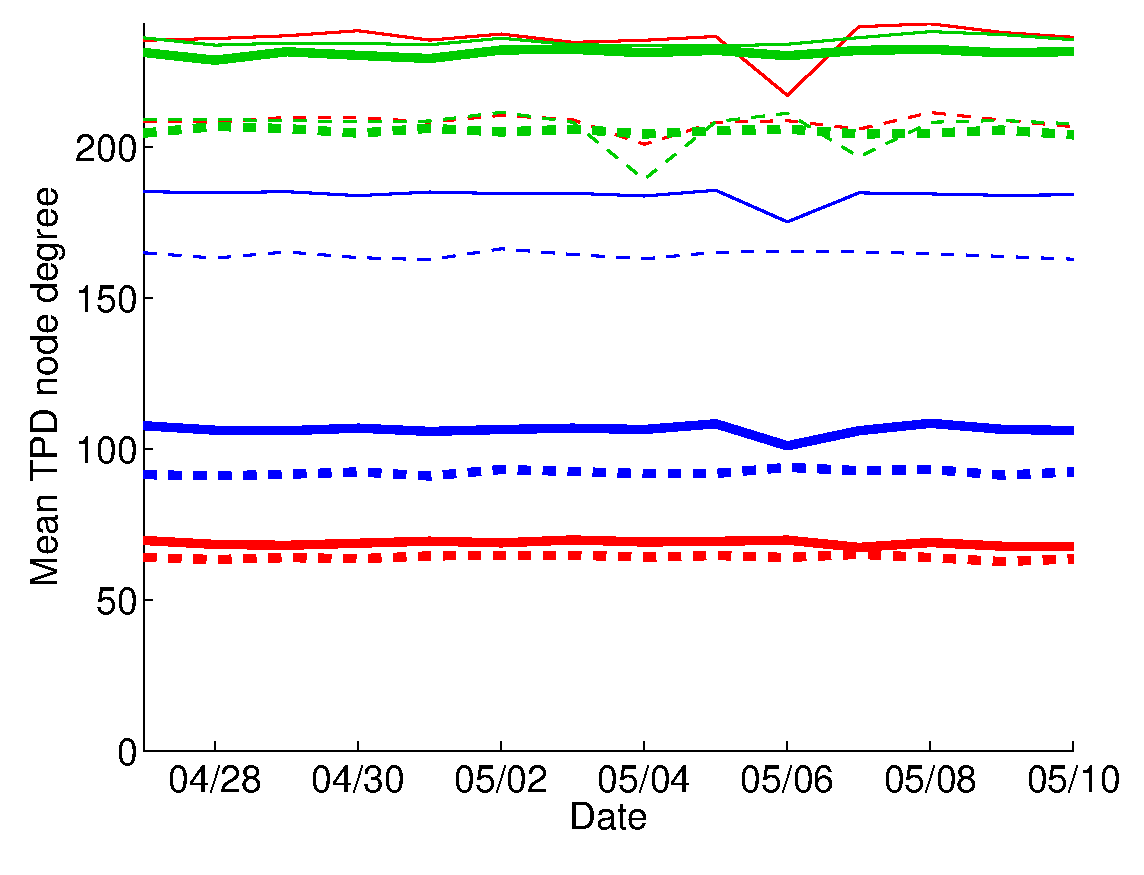
\includegraphics[width=\textwidth]{figures/plots/third-mean-top10-entities.eps}
    \caption{Mean value of the degree of the 10 most-connected TPD nodes, $V_T$ over time for each user profile $U$}
    \label{fig:third_mean_top10_with_entities}
  \end{subfigure}

  \caption{Time evolution of the first and third-party degree metrics for the most-connected FPD and TPD nodes, accordingly \textbf{\textit{without}} (left) and \textbf{\textit{with}} (right) domain grouping according to entities.}
  \label{fig:highest_degree_nodes}

  \end{figure*}


\subsubsection{Result evaluation}

\textbf{Metrics \textit{without} entity grouping (Figure \ref{fig:metrics_without_entities}):} As depicted in Figures \ref{fig:first_means} and \ref{fig:third_means}, the user profiles \textit{Ghostery\_Default} and \textit{NoAdblocker} have the worst performance, since the first parties they visit load the highest mean number of third parties. Although we would expect that the use of an adblocker, such as Ghostery, should provide us with better results, a closer look at its initial settings show that the adblocker functions as a third-party tracker that does not block any third parties by default, unless configured appropriately. The metric has a consistently but only slightly lower value for the profile \textit{NoAdblocker\_DNT}.

A steadily better performance is to be noted for the user profiles with the exact same settings as above, but with a Mobile User Agent, i.e. \textit{Ghostery\_Default\_MUA}, \textit{NoAdblocker\_MUA} and \textit{NoAdblocker\_DNT\_MUA}, where the mean node degree is markedly lower and the relative order of the three profiles remains unaltered.

An improvement in the results comes with the use of AdblockPlus, since the profiles \textit{Adblockplus\_Default} and \textit{Adblockplus\_Default\_MUA} using AdblockPlus with its default settings have a mean node degree significantly lower than the aforementioned worst cases. This observation is particularly important, because it indicates the advantage of using an adblocker, even with minimal settings --but not disabled, as in the case of \textit{Ghostery\_Default}.

Nevertheless, the most efficient user profiles from an adblocking viewpoint are, unsurprisingly, the ones that have an adblocker installed and configured to a maximal-protection level. In this case, a mean node degree up to nearly 80\% lower is achieved with respect to the default case, while to be pointed out is the constantly better performance of Ghostery with respect to AdblockPlus, when both are compared under equal terms, that is, manual settings to achieve an optimal result.

An inspection of the graph-density results for each of the profiles under scrutiny yields almost the same results, albeit the use of Mobile User Agent seems to deteriorate the performance, unlike the previous cases. The reason behind this behavior is that from all of the third parties that were loaded under a Desktop User Agent, only the most popular ones are still loaded under a Mobile User Agent, i.e. the ones that have a higher chance of being requested by more first parties, such as \texttt{doubleclick.net}. This leads to a more connected graph despite the lower degree of each of its nodes.

\textbf{Metrics \textit{with} entity grouping (Figure \ref{fig:metrics_with_entities}):} We now enhance the graphs $G$ that correspond to each user profile $U$ with information regarding the logical entity they belong to, as described in Section \ref{sec:logical_entity} and group multiple TPD nodes into one supernode representing their common administrative organization.

Looking at the Figure \ref{fig:metrics_with_entities} where this logical-entity information has been taken into account and juxtaposing it to Figure \ref{fig:metrics_without_entities}, we observe that the mean FPD node degree is reduced, while on the other hand, no considerable changes are to be observed for the mean TPD node degree or the graph density. As far as the relative ad-blocking efficiency of the user profiles is concerned, we should remark that this does not present any change with respect to the results before entity grouping had been applied.

\textbf{Highest-degree domains (Figure \ref{fig:highest_degree_nodes}):} After an examination of the Figure \ref{fig:highest_degree_nodes}, we observe that in the worst case, a first-party website can be tracked by up to 170 third parties (Figure \ref{fig:first_mean_top1_without_entities}), whilst a third-party can have access and collect information about our browsing behavior from almost 500 first-party websites that we visited (Figure \ref{fig:third_mean_top1_without_entities}). However, it is important to mention that the performances of the user profiles $U$ remain approximately in the same relative order as in the previously analyzed cases, with the use of the adblockers to considerably enhance the user's protection against tracking. Of course the results are now expected to present higher variations and thus be less accurate, since the values are now not averaged at all or averaged on 10 values, accordingly.

\textbf{Graph separation (Figure \ref{fig:top_last_domains_comparison}):} In order to investigate whether the ad-blocking tools have been subject to optimizations that would enable better performances for the top-visited domains, our URL sample set $W$ includes, as explained in Section \ref{sec:crawled_urls}, an additional set of 500 domains with a rank uniformly selected between 500 - 1M from the Alexa Top Rank. To this end, we separate the original graph $G$ into two independent graphs $G_T$ and $G_R$ for the 500 top-visited and the 500 uniformly-selected URLs, respectively, and followingly directly compare their performances.

The graph provides a direct comparison of the ad-blocking efficiency of the user profiles $U$ for the two URL subsets. Unsurprisingly, the relative performance of the different profiles remains roughly unaffected. Nonetheless, the efficiency on the last 500 domains yields better results, with the mean FPD node degree to be considerably and consistently lower than the one calculated for the top 500 domains.


\textbf{Correlation (Figure \ref{fig:first_party_degree_relative_rank}):} Another index of whether the aforementioned hypothesis holds true can be provided by the correlation between the rank of the URL and a performance metric --i.e. the FPD node degree. In Figure \ref{fig:first_party_degree_relative_rank} the FPD node degree has been plotted with respect to the domain rank to provide a finer visualization of the previous result, for a specific user profile $U$ and a specific date. The figure presents only the data for the top 500-ranked websites. As results from the graph, the points do not show any trend that can suggest a clear relationship between the relative rank and the node degree.

Our visual observation is confirmed by the calculation of the correlation of the two parameters that yields 10.49\%.


\textbf{CDF (Figure \ref{fig:cdf_first_node_degree}):} Examining the cumulative distribution function (CDF) of the FPD node degree we can profile the extent to which the visited URLs are being tracked by third party domains. We plot the probability $$P(\textnormal{FPD node degree} \leq X)$$ of a FPD node to have a degree less than $X$ or, equivalently, to load less than $X$ TPDs when no adblocker is used (user profile \textit{NoAdblocker}) for a specific date. In order to investigate the effect of the rank on the CDF, we plotted the results for the FPD nodes of the whole URL sample set, the top-ranked 500 URLs and the uniformly-selected ones, respectively.

As can be seen, about 20\% of the websites loaded almost no third parties, while at the same time only a very limited number were accessed by more than 50 TPD nodes in all cases. Comparing the curves, we conclude again that less third parties were loaded for the uniformly-selected domains, affirming the results extracted from Figure \ref{fig:top_last_domains_comparison}.


    \begin{figure}
   \centering

  \begin{subfigure}{.45\textwidth}
    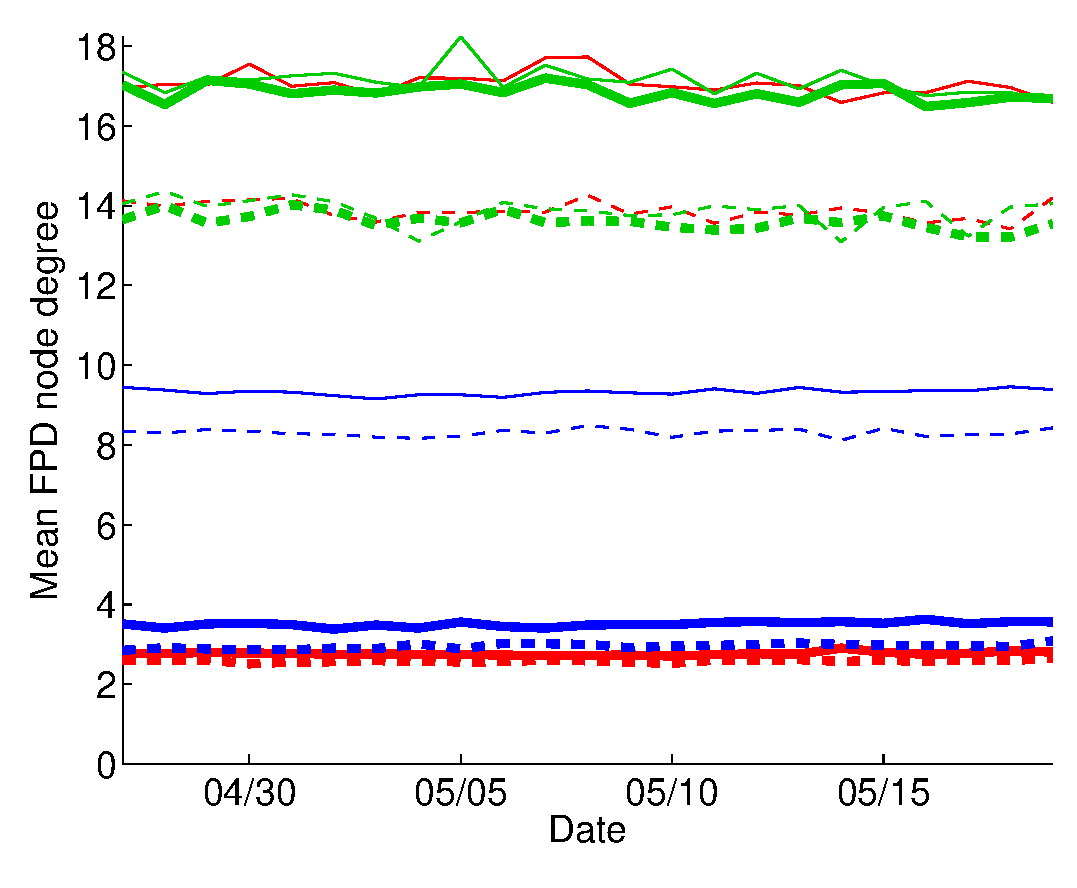
\includegraphics[width=\textwidth]{figures/plots/top500-first-means.eps}
    \caption{Mean value of the degree of the 500 top-visited FPD nodes}
    \label{fig:top500_first_means}
  \end{subfigure}

  \begin{subfigure}{.45\textwidth}
    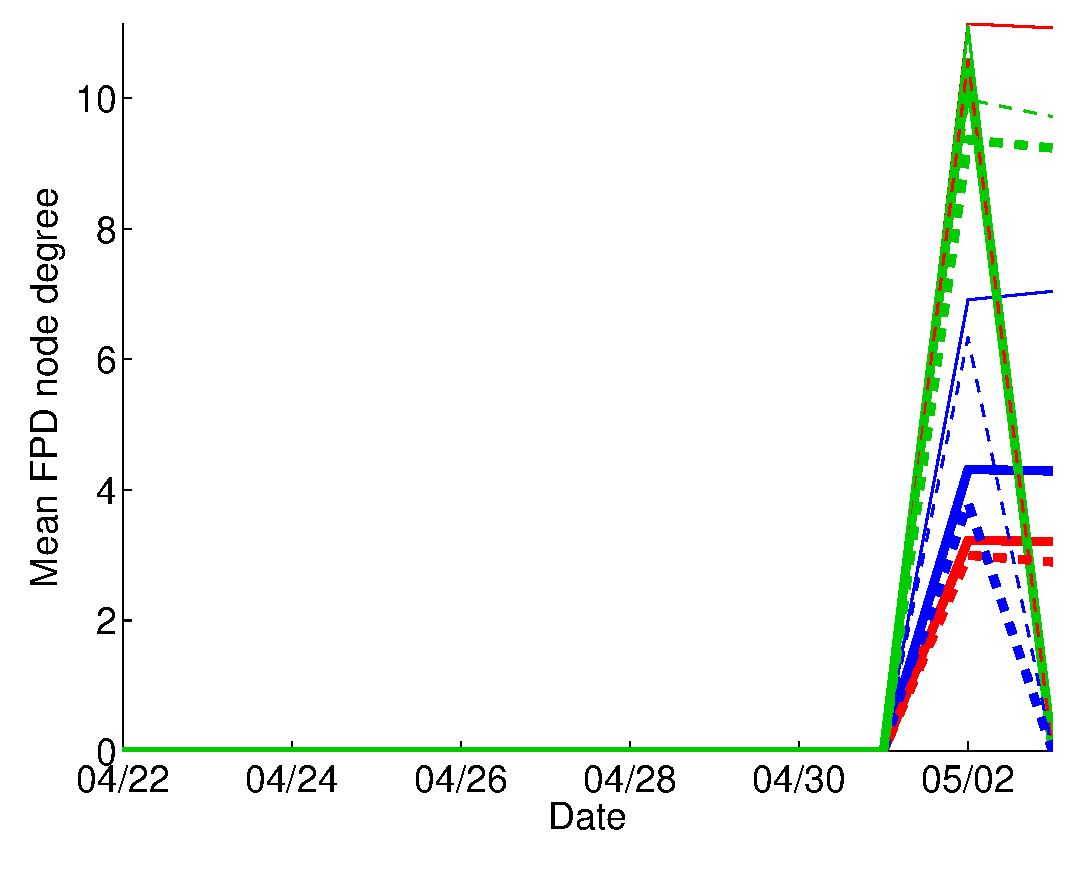
\includegraphics[width=\textwidth]{figures/plots/last500-first-means.eps}
    \caption{Mean value of the degree of the 500 uniformly-selected FPD nodes}
    \label{fig:top500_random_means}
  \end{subfigure}
  \caption{Comparison of the performance of the user profiles $U$ when tested the top-visited domains and the uniformly-selected ones.}
  \label{fig:top_last_domains_comparison}
  \end{figure}

  \begin{figure}
 \centering
 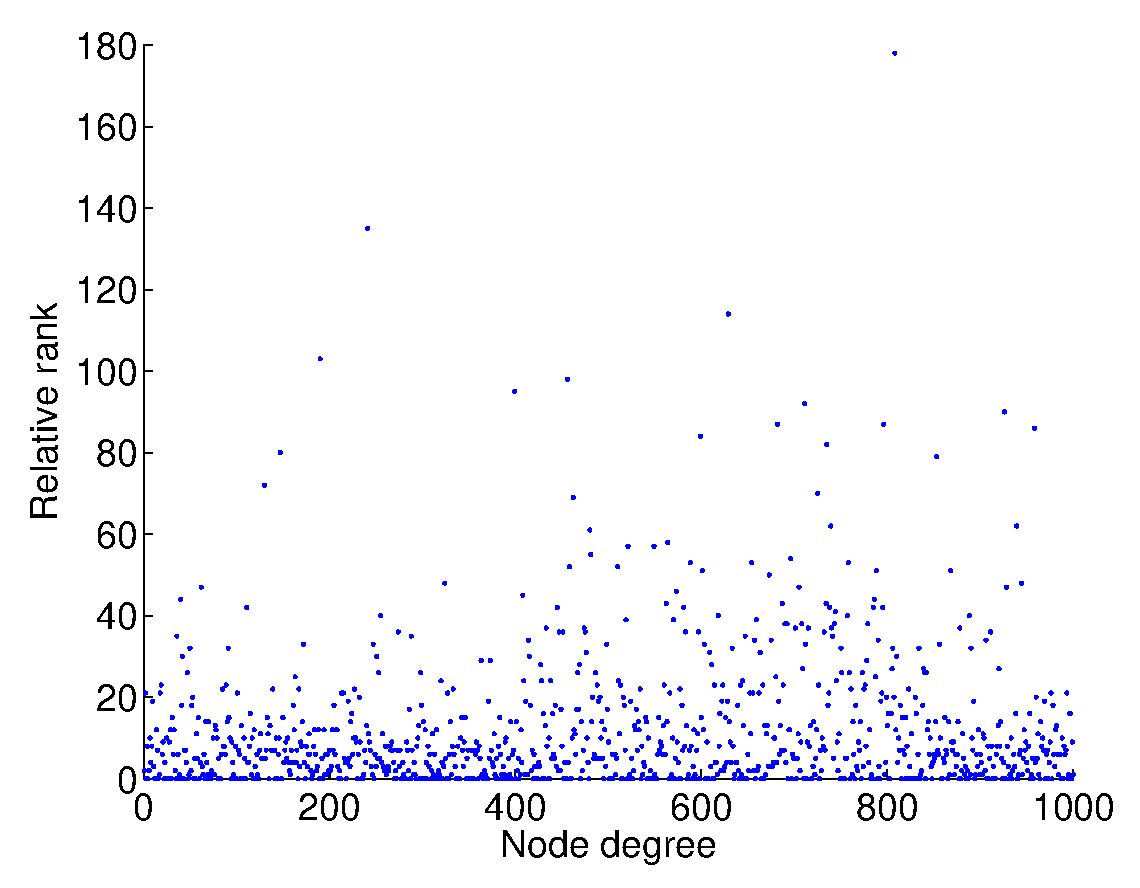
\includegraphics[width=.45\textwidth]{figures/plots/scatterplot.eps}
 \caption{FPD node degree against FPD relative rank for the profile \textit{NoAdblocker} on 20/05/2016}
 \label{fig:first_party_degree_relative_rank}
\end{figure}

\begin{figure}
 \centering
 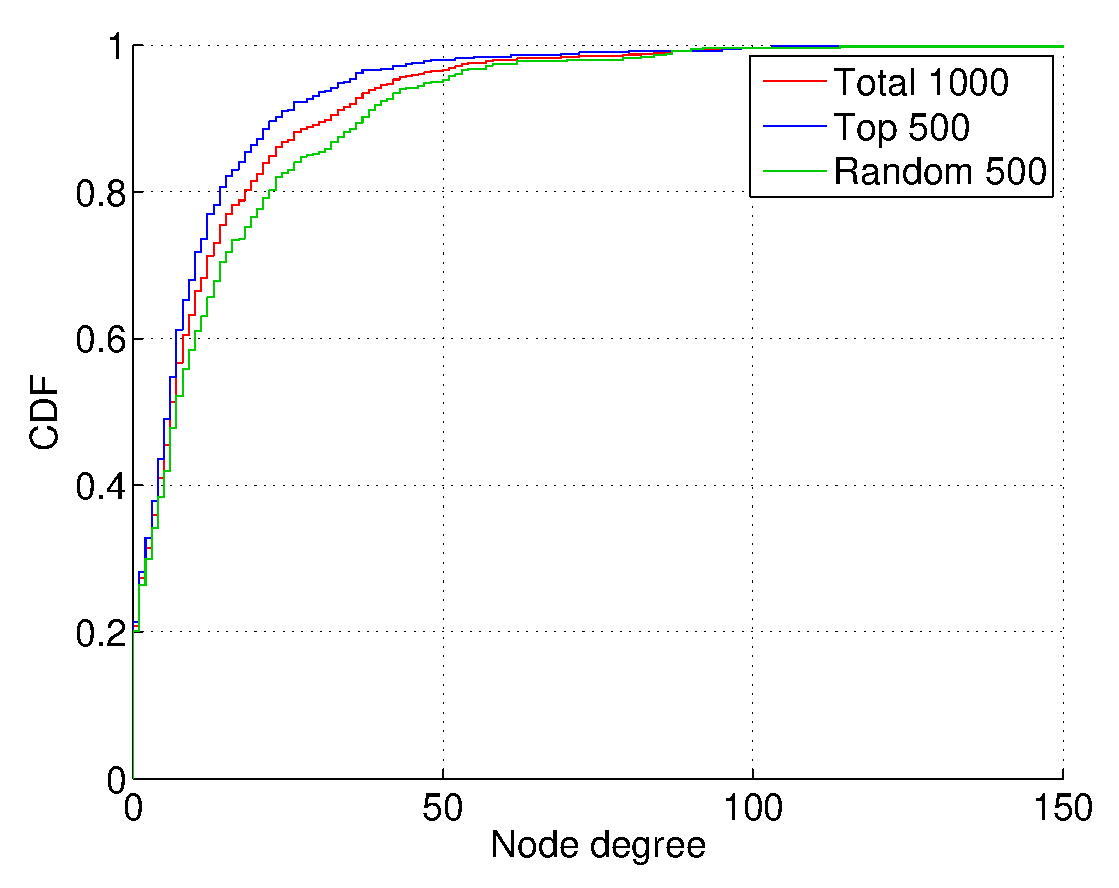
\includegraphics[width=.45\textwidth]{figures/plots/cdf-first-node-degree.eps}
 \caption{Cumulative distribution function of FPD node degree for the profile \textit{NoAdblocker} on 20/05/2016}
 \label{fig:cdf_first_node_degree}
\end{figure}

\subsubsection{Metric evaluation}
Notwithstanding that the relative performance of the user profiles remained practically unaltered with the use of the different metrics, as illustrated above, the discrepancies between the results of the profiles are not always trivial to tell apart. As a consequence, the mean TPD node degree is less suitable than the mean FPD node degree when profiles with smaller efficiency differences are to be discerned, while their distignuishability weakens markedly further when the graph density is used as a metric.


\subsection{Influence of profile parameters}
As explained in \ref{sec:user_profiles}, the user profiles $U$ are created as a combination of different parameters that needed to be scrutinized. After a thorough examination of the experimental results of the previous sections, the impact of these parameters can be summarized as follows:

\textbf{Adblocker installed:} As experimentally confirmed, the use or no use of an adblocker is the most decisive factor when it comes to being tracked by third parties, since even with the minimal-protection settings, the mean first-party node degree can improve by up to 40\%. The profiles with Ghostery installed under default settings have to be excluded from this analysis, however, since Ghostery has its adblocker functionality initially disabled, as discussed above. Additionally, the selection of the adblocker can also play an important role, as the comparison of the Ghostery and AdblockPlus under maximal-proteciton settings indicated.

\textbf{Block policy:} The block policy configured for each adblocker is of crucial importance, as results from the considerable contrasts between the profiles with default and maximal-protection policies --an improvement of almost 80\% and 50\% was achieved in the mean first-party degree for Ghostery and AdblockPlus, respectively.

\textbf{Do Not Track header:} The reason that the influence of this parameter is not as notable as in the other cases is the fact that the browser user has no control over whether the DNT flag is honored or not and hence websites and advertisers may either obey or completely ignore it.

\textbf{Mobile User Agent:} Websites that received requests by a mobile user agent indeed responded with a considerably lower number of third parties. A plausible explanation for this behavior is the requirement for less bandwidth that the mobile websites usually conform to. As a consequence of this limitation, less content is loaded and hence less requests are sent to third parties. This discrepancy was of course less obvious for the user profiles with maximal protection enabled, since tracking by third parties is already reduced.

\subsubsection{Blacklist latency}
{\color{red}Can you add the study of when the blacklists are updated?}

\subsection{Geographical impact}

Another interesting finding after the execution of our experiments and the entity analysis is the classification of the third parties according to their geographical location. With the entity data extracted from WHOIS, we assign a country to each third-party domain (TPD node) of the request graphs and visualize the comparison between the different countries on the world map in Figure \ref{fig:third_party_map}. The darkest regions (blue) are the countries with the most TPDs loaded, while the white ones host none of the TPDs found in our graphs.

As we would expect, the USA and China host most of the third-party domains loaded, while regions such as Africa or Latin America contain very few TPDs.

\begin{figure*}
 \centering
 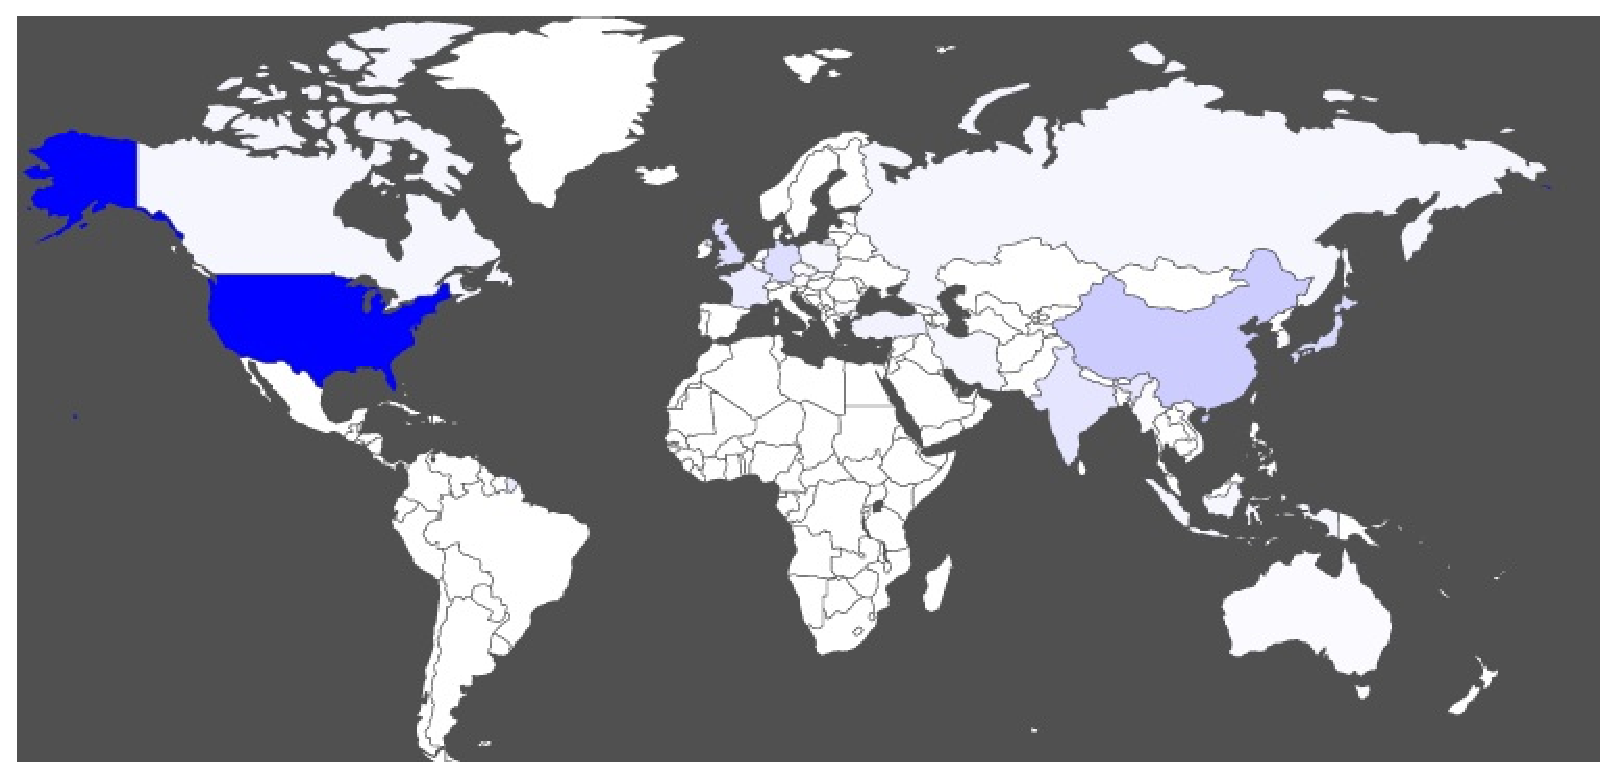
\includegraphics[width=\textwidth]{figures/third_party_map.eps}
 \caption{World map depicting the locations of the third parties loaded during our experiments.}
 \label{fig:third_party_map}
\end{figure*}


\subsection{Logical entity}

As seen above, grouping the TPD nodes according to the logical entities they belong to brings a considerable reduction of the mean FDP node degree, asserting that the number of logical entities potentially collecting information about the user is indeed less than that of the actual third-party domains tracking them.

On the contrary, the mean TPD node degree, as well as the graph density do not present any significant variation, which leads us to the conclusion that the various logical entities have on average access to roughly the same first parties, although controlling multiple third-party domains.

Table \ref{table:top_10_tpd_entities} summarizes the 10 entities with the highest TPD node degree, i.e. that were present on most of the visited URLs when the default Browser settings were applied (\textit{NoAdblocker}) and for a specific date.

\begin{table}
  \centering
  \begin{tabular}{|c|c|c|}
  \hline
  No. & Logical Entity & Degree [\%] \\
  \hline
  1 & Google Inc. & 674 \\
  2 & Facebook Inc. & 323 \\
  3 & Domains By Proxy LLC & 206 \\
  4 & AppNexus Inc. & 156 \\
  5 & TMRG Inc. & 145 \\
  6 & Twitter Inc. & 136 \\
  7 & Oracle Corporation & 120 \\
  8 & Yahoo! Inc. & 111 \\
  9 & Adobe Systems Incorporated & 99 \\
  10 & The Rubicon Project Inc. & 94 \\
  \hline
  \end{tabular}
  \caption{Logical entities with the highest TPD node degree for user profile \textit{NoAdblocker} on 20/05/2016}
  \label{table:top_10_tpd_entities}
  \end{table}

\subsection{Rank impact}

In Figures \ref{fig:top_last_domains_comparison} and \ref{fig:cdf_first_node_degree} we investigated the relationship between the URL rank and the FPD node degree. As resulted from the plot of the mean FPD node degree, the uniformly-selected FPD nodes were accessed on average by less third parties with respect to the top-ranked 500 FPD nodes, thus contradicting our initial assumption. On the other hand, a higher number of loaded third parties can be justified, if the size and the popularity of the first domains is taken into consideration, as opposed to that of the last domains.

Another observation can be made when the correlation between the rank and the FPD node degree is examined. More specifically, the rank of each website among the top 500 of the rank (Figure \ref{fig:first_party_degree_relative_rank}) does not present a strong correlation to the number of third parties it loaded, hence reinforcing our conclusion above.

\section{Related work}

\textit{Pujol et al} in \cite{pujol} aim to infer the use or no use of an adblocker by examining the HTTP(S) requests sent by a browser, using the ratio of the ad requests and the downloads of filter lists as indicators. Moreover, the performance of 7 different user profiles --adblocker-configuration combinations-- is compared based upon the total number of unblocked requests per user profile. Furthermore, although the ad traffic is examined through the analysis of the number of requests at different time instances throught the day, the content-type of the ad requests, as well as the effect of enabling non-intrusive ads, no long-term data is collected regarding the tracking behavior of the third parties.

\textit{Ruffell et al} in \cite{ruffel2015} analyze the effectiveness of various browser add-ons in mitigating and protecting users from third-party tracking networks. In total 7 user profiles are created, each with a different combination of multiple add-ons and browser settings, and each of the profiles visits the 500 top Alexa Rank websites, while the HTTP request data is recorded with the use of Mozilla Lightbeam. The data is collected for one crawling cycle and followingly the efficiency analysis is performed based upon various graph metrics. Nevertheless, none of these user profiles examines the difference of the effect of the third-party tracking on devices with Mobile User Agents.

\textit{Mayer and Mitchell} implemented in \cite{mayer} the tool FourthParty --an open-source platform for measuring dynamic web content-- as an extension to Mozilla Firefox. Afterwards, they created several user profiles, so as to test the efficiency of different adblocking tools under certain settings (blacklists) and crawled the 500 top Alexa websites three times using FourthParty, in order to extract the average decrease in tracking with the use of the ad-blocking tools. The results of such an analysis may, however, be subject to biases, since the URL sample set used has been vastly examined in the bibliography so far and many adblockers may have been optimized to provide a higher efficiency when tested against it.

%NSDI 2013 Google, alexis
%Advertisement bidding
%ublock.org is a lightweight blocking proxy
%https://trackography.org/

\section{Conclusions} \label{sec:conclusions}

\bibliographystyle{plain}
\bibliography{relatedwork}
\end{document}
